\documentclass[12pt,a4paper]{report}

\usepackage{styles/dolgozat}

\usepackage{listings}
\usepackage{float}
\usepackage{styles/cpp}
\usepackage{styles/python}
\usepackage{styles/java}

\usepackage{hyperref}

\begin{document}

\pagestyle{empty} %a címlapon ne legyen semmi=empty, azaz nincs fejléc és lábléc

% A Miskolci Egyetem címere
{\large
\begin{center}
\vglue 1truecm
\textbf{\huge\textsc{Szakdolgozat}}\\
\vglue 1truecm

\includegraphics[width=4.8truecm, height=4truecm]{images/me_logo.png}\\
\textbf{\textsc{Miskolci Egyetem}}
\end{center}}

\vglue 1.5truecm %függõleges helykihagyás

% A szakdolgozat címe, akár több sorban is
{\LARGE
\begin{center}
\textbf{Tesztelési módok szerepe és jelentősége a szoftverfejlesztési folyamatokban}
\end{center}}

\vspace*{2.5truecm}
% A hallgató neve, évfolyam, szak(ok), a konzulens(ek) neve
{\large
\begin{center}
\begin{tabular}{c}
\textbf{Készítette:}\\
Orosz Dénes Milán\\
Programtervező informatikus
\end{tabular}
\end{center}
\begin{center}
\begin{tabular}{c}
\textbf{Témavezető:}\\
Piller Imre\\
\textbf{Konzulens:}\\
Albert Laura
\end{tabular}
\end{center}}
\vfill
% Keltezés: Hely, év
{\large
\begin{center}
\textbf{\textsc{Miskolc, 2022}}
\end{center}}

\newpage


\newpage

\pagestyle{empty}

%Feladatkiiras
\begin{flushleft}
\textsc{\bfseries Miskolci Egyetem}\\
Gépészmérnöki és Informatikai Kar\\
Alkalmazott Matematikai Intézeti Tanszék\hspace*{4cm}\hfil \textbf{Szám:}
\end{flushleft}
\vskip 0.5cm
\begin{center}
\large\textsc{\bfseries Szakdolgozat Feladat}
\end{center}
\vskip 0.5cm
Orosz Dénes Milán (HC1Y8Y) programtervező informatikus jelölt részére.\newline

\noindent\textbf{A szakdolgozat tárgyköre:} Szoftvertechnológia \newline

\noindent\textbf{A szakdolgozat címe:} Tesztelési módok szerepe és jelentősége a szoftverfejlesztési folyamatokban\newline

\noindent\textbf{A feladat részletezése:}

\medskip

\emph{A tesztelés a szoftverfejlesztési folyamat egészére nézve kiemelt jelentőséggel bír. A dolgozat azt mutatja meg, hogy mikor, milyen célból, milyen fajta tesztek készítésére és használatára van szükség.}

\medskip

\emph{Ehhez az alapot egy olyan alkalmazás elkészítése adja, amely igyekszik minden, tesztelés, tesztelhetőség szempontjából fontos területet lefedni, beleértve az adatbáziskezelést és a felhasználói felület megvalósítását. Ezen keresztül mutatja be a szoftvertesztelés fajtáit, lépéseit, az egyes fázisokon belül alkalmazott módszereket. Az alkalmazás elkészítéséhez Java programozási nyelv kerül felhasználásra.}

\vfill

\noindent\textbf{Témavezető:} Piller Imre (tanársegéd) \newline

\noindent\textbf{Konzulens:} Albert Laura (független tesztelési szakértő)\newline

\noindent\textbf{A feladat kiadásának ideje:} 2022. Miskolc\newline

%\noindent\textbf{A feladat beadásának határideje:}

\vskip 2cm

\hbox to \hsize{\hfil{\hbox to 6cm {\dotfill}\hbox to 1cm{}}}

\hbox to \hsize{\hfil\hbox to 3cm {szakfelelős}\hbox to 2cm{}}

\newpage

\vspace*{1cm}  
\begin{center}
\large\textsc{\bfseries Eredetiségi Nyilatkozat}
\end{center}
\vspace*{2cm}  

Alulírott \textbf{Orosz Dénes Milán}; Neptun-kód: \texttt{HC1Y8Y} a Miskolci Egyetem Gépészmérnöki és Informatikai Karának végzős Programtervező informatikus szakos hallgatója ezennel büntetőjogi és fegyelmi felelősségem tudatában nyilatkozom és aláírásommal igazolom, hogy \textit{Tesztelési módok szerepe és jelentősége a szoftverfejlesztési folyamatokban}
című szakdolgozatom saját, önálló munkám; az abban hivatkozott szakirodalom
felhasználása a forráskezelés szabályai szerint történt.\\

Tudomásul veszem, hogy szakdolgozat esetén plágiumnak számít:
\begin{itemize}
\item szószerinti idézet közlése idézőjel és hivatkozás megjelölése nélkül;
\item tartalmi idézet hivatkozás megjelölése nélkül;
\item más publikált gondolatainak saját gondolatként való feltüntetése.
\end{itemize}

Alulírott kijelentem, hogy a plágium fogalmát megismertem, és tudomásul veszem, hogy
plágium esetén szakdolgozatom visszautasításra kerül.

\vspace*{3cm}

\noindent Miskolc, \hbox to 2cm{\dotfill} .év \hbox to 2cm{\dotfill} .hó \hbox to 2cm{\dotfill} .nap

\vspace*{3cm}

\hspace*{8cm}\begin{tabular}{c}
\hbox to 6cm{\dotfill}\\
Hallgató
\end{tabular}



\newpage

\noindent 1.

\begin{tabular}{cl}
&szükséges (módosítás külön lapon) \\
A szakdolgozat feladat módosítása& \\
& nem szükséges\\
&\\
\hbox to 4cm{\dotfill}&\multicolumn{1}{c}{\hbox to 5cm{\dotfill}}\\
dátum& \multicolumn{1}{c}{témavezető(k)}
\end{tabular}
\vskip1.5mm

\noindent 2. A feladat kidolgozását ellenőriztem:

\vskip1.5mm

\begin{tabular}{l@{\hspace*{4cm}}l}
témavezető (dátum, aláírás):& konzulens (dátum, aláírás):\\
\dotfill&\dotfill\\
\dotfill&\dotfill\\
\dotfill&\dotfill
\end{tabular}

\vskip1.5mm

\noindent 3. A szakdolgozat beadható:

\vskip1.5mm

\begin{tabular}{@{\hspace*{1.3cm}}c@{\hspace*{2.1cm}}c}
\hbox to 4cm{\dotfill}&\multicolumn{1}{c}{\hbox to 5cm{\dotfill}}\\
dátum& \multicolumn{1}{c}{témavezető(k)}
\end{tabular}

\vskip1.5mm

\noindent 4.
\begin{tabular}[t]{@{}l@{\hspace*{1mm}}l@{\hspace*{1mm}}l@{}}
A szakdolgozat& \hbox to 3.5cm{\dotfill} &szövegoldalt\\
              & \hbox to 3.5cm{\dotfill} &program protokollt (listát, felhasználói leírást)\\
              &\hbox to 3.5cm{\dotfill}   &elektronikus adathordozót (részletezve)\\
              &\hbox to 3.5cm{\dotfill} & \\
              &\hbox to 3.5cm{\dotfill} &egyéb mellékletet (részletezve)\\
              &\hbox to 3.5cm{\dotfill} &\\
\end{tabular}
\newline tartalmaz.

\vskip1.5mm

\begin{tabular}{@{\hspace*{1.3cm}}c@{\hspace*{2.1cm}}c}
\hbox to 4cm{\dotfill}&\multicolumn{1}{c}{\hbox to 5cm{\dotfill}}\\
dátum& \multicolumn{1}{c}{témavezető(k)}
\end{tabular}

\noindent 5.

\begin{tabular}{ll}
&bocsátható\\
A szakdolgozat bírálatra& \\
& nem bocsátható\\
\end{tabular}

\vskip1.5mm

\noindent A bíráló neve: \hbox to 8cm{\dotfill}

\vskip4mm

\begin{tabular}{@{\hspace*{1.3cm}}c@{\hspace*{2.1cm}}c}
\hbox to 4cm{\dotfill}&\multicolumn{1}{c}{\hbox to 5cm{\dotfill}}\\
dátum& \multicolumn{1}{c}{szakfelelős}
\end{tabular}

\noindent 6.
\begin{tabular}[t]{@{}l@{\hspace*{1mm}}l@{\hspace*{1mm}}l@{}}
A szakdolgozat osztályzata& &\\
&a témavezető javaslata:& \hbox to 3cm{\dotfill}\\
&a bíráló javaslata:& \hbox to 3cm{\dotfill}\\
&a szakdolgozat végleges eredménye:& \hbox to 3cm{\dotfill}
\end{tabular}

\vspace*{4mm}

\noindent Miskolc, \hbox to 4.5cm{\dotfill} \hspace*{2.5cm}
\begin{tabular}[t]{cc}
\hbox to 6cm{\dotfill}\\
a Záróvizsga Bizottság Elnöke
\end{tabular}


\cleardoublepage
\pagenumbering{gobble}
\tableofcontents
\cleardoublepage
\pagenumbering{arabic}

\newpage

\pagestyle{fancy}

\Chapter{Bevezetés}



Maga a tesztelés a szoftverfejlesztési folyamatnak egy nagyon fontos része. Mindenki tapasztalt már hasonlót, hogy egy program nem úgy működött, ahogy annak kellett volna. Ez a hibás működés legyen az bármennyire kis mértékű, nagy időbeli és pénzbeli veszteségeket okozhat egy cégnek, sőt akár fizikai sérüléssel is járhat a jelenlegi szituációtól függően. A szoftvertesztelés lényege, hogy minimálisra csökkentse a kockázatát annak, hogy egy szoftver működés közben meghibásodik, illetve ellehetetlenítse egy olyan szoftver kiadását, amiben ismert hiba van, miközben lehetőséget ad a szoftverminőség kiértékelésére.

Ha valaki a meghallja a szoftvertesztelés szót, akkor gyakran tesztek írására és futtatására gondol, pedig maga a szoftvertesztelés egy teljes folyamat számos lépéssel, aminek csak egy része a teszt esetek megírása és az eredmények ellenőrzése.

Hasonlóan tévhit, hogy a szoftvertesztelés, csak a felhasználók által megszabott követelmények verifikációjára fókuszál, ugyanis bármilyen meg szabott speciális követelménynek való megfelelést is tartalmaznia kell, illetve a validációt is, ami már a működési környezetben ellenőrzi az igényeket.

Bármely projekt esetén a tesztelés céljai az alábbiak lehetnek:
\begin {enumerate}
 \item A munkatermékek, mint például a követelmények, felhasználói történetek, műszaki tervek és kód hibamegelőzés céljából történő kiértékelése

\item Annak igazolása, hogy az összes meghatározott követelmény teljesült-e


\item Annak ellenőrzése, hogy a teszt tárgya teljes mértékben implementálásra került, továbbá annak, validálása, hogy a felhasználók, illetve más érintett felek elvárásainak megfelelően működik.

\item A teszt tárgyának minőségébe vetett bizalom kiépítése

\item A meghibásodások és hibák megtalálása és ezáltal a nem megfelelő szoftverminőség kockázati szintjének csökkentése

\item Megfelelő információ biztosítása az érintett feleknek, hogy ezáltal megalapozott döntést hozhassanak különösen a teszt tárgyának minőségi szintjére vonatkozóan

\item A szerződésben foglalt, jogi vagy szabályozott követelményeknek, szabványoknak való megfelelés biztosítása, és/vagy igazolni a teszt tárgyának ezen követelményeknek, szabványoknak való megfelelőségét
\end {enumerate}
A tesztelés céljai változhatnak a tesztelt komponens vagy rendszer, a tesztszint és a szoftverfejlesztési életciklusmodell kontextusától függően\cite{syllabus}.


A szoftvertesztelés számos fajtával rendelkezik. Attól függően, hogy mi tartozik a tesztelés hatókörébe, különbséget teszünk a tesztelési fajták között. A szakdolgozat célja ezeknek a fajtáknak a leírása és bemutatása tesztelési környezetben, illetve környezet nélkül, amennyiben arra van lehetőség.

\Chapter{Koncepció}

\Section{A fejezet célja}
A tesztelési módszerek csoportosítására több módszer is lehetséges, viszont fontos tudni, hogy optimális esetben többet is használunk a tesztelés különböző szintjein. Én manuális, ad-hoc, szisztematikus és fekete doboz tesztelési módszereket fogok alkalmazni a programomon.\\
A szakdolgozat folyamán többször is fogom használni a szkript szót. Ez alatt azt a lépéssorozatot értem, amiben le van írva, hogy az adott tesztet, hogyan kell elvégezni, milyen előfeltételek vannak és mi az elvárt eredmény.

\Section{Tartalom és felépítés}

Mielőtt a négy módszerre részletesen kitérnék és szakirodalmakkal, illetve kutatásokkal bővíteném ki, szükségesnek érzem ezeknek a magyarázatát.
\begin{itemize}

\item Manuális (kézi) tesztelés: A tesztelést a gép helyett egy ember végzi, aki  hibákat keres akár a működésbe, akár egy teszt szkriptbe, de ilyenkor még a szubjektív hibákat is látócső alá lehet venni.

\item Ad-hoc tesztelés: Ad-hoc tesztelés alatt akár a szabad tesztelést is nevezhetjük. Ez a mód igazából nem szab korlátot és utat sem mutat a tesztelő számára. Teljes mértékben a tesztelő kezében van, hogy milyen módszereket használva teszteli az adott szoftvert.

\item Szisztematikus tesztelés: A szisztematikus tesztelés az ad-hoc fordítottja. Ebben a módszertanban egy előre definiált módszerrel és tesztesettel tekintünk a szoftverre és mindig pontosan azt a funkció működését ellenőrizzük amire a teszt eset íródott.

\item Fekete doboz tesztelés: Fekete doboz tesztelés alatt egy olyan módszertant értünk, ahol magát a szoftver belső működését vagy nem ismerjük, vagy ignoráljuk, ugyanis nekünk csak az számít, hogy egy adott bemenetre adott kimenetet kapjunk.
\end{itemize}

\Section{Tesztelési módszertanok és módszerek}
A szoftvertesztelés módszertanaival már nagyon sok ember foglalkozott, bár többnyire az elkészült irodalmak egy-egy módszertant említenek specifikusan, vagy talán kettő ellentmondását vagy az együtt használás előnyeit mutatják be. Fontos tudni, hogy minél több módszer kerül használatra egy szoftver tesztelése közbe, annál nagyobb lefedettséget biztosít és annál kisebb lesz az esély arra, hogy hiba marad a programunkba.

\subsection{Manuális tesztelés} A manuális tesztelést tekinthetjük a módszertanok közül a legegyszerűbbnek. Ha valaki a teszteléssel szeretne foglalkozni, mindig ezzel fogja kezdeni és nem feltételezi azt sem a szakma, hogy IT végzettséggel rendelkezzen valaki, elég ha van hozzá affinitása. Természetesen ha valakinek már végzettsége van, az nagyon megkönnyíti a munkát, de így sem elvárható, hogy rögtön egy hét után már önállóan hiba nélkül tudjon dolgozni a tesztelő. A legegyszerűbb módszertannak neveztem az előbb, mégis tudni kell hogy a legszínesebb is tud egyszerre lenni, ugyanis cégenként változik a bevált módszer és a feladatkör.\\
Az esetek többségében a folyamat úgy zajlik, hogy a tesztelő megkapja a tesztforgatókönyvet a projekt- vagy tesztkoordinátortól, szenior tesztelőtől, amelyben tételesen le van írva, miket kell vizsgálnia, mi az elvárt eredmény, és amennyiben nem a várt eredményt kapja, akkor mi a teendő. Ez lehet olyan triviális apróság, mint például hogy funkcionális tesztelésnél az adott gombra kattintva nem történik semmi, vagy lefagy a rendszer, nem a megfelelő oldal nyílik meg stb. A tesztelő munkája nem attól izgalmas, hogy nem talál hibát, hanem attól, ha minél többet fedez fel\cite{computerworld}.\\
A szakma és a módszertan legizgalmasabb része maga a hiba felderítése és nyomozása. 
\begin{itemize}
\item Mi az ami a hibát okozza?
\item Hogy lehet reprodukálni?
\item A kód melyik részében található?
\end{itemize}
Ezeknek a kérdéseknek a megválaszolásával jutunk el oda, hogy a manuális tesztelő megírja a riportot a hibáról és továbbítja a fejlesztőknek.\\
Ehhez viszont az adott szoftvert, annak funkcióit alaposan ismerni kell (az újat és a régit egyaránt). Ezért a junior manuális tesztelők az első 2-6 hónapban rengeteg dokumentációt olvasnak (ha van), munkájuk nagy részét felületi tesztek teszik ki, hogy minél jobban meg tudják ismerni a rendszereket. Akinek már van elég tapasztalata, annak a napi munka részét képezi a bug-tracking (a felfedezett hiba nyomon követése), a tesztmódszertan kidolgozása, a tesztesetek (újra)definiálása, a tesztforgatókönyv-készítés és a log elemzés is\cite{computerworld}.


\subsection{Ad-hoc tesztelés} A manuális tesztelés alatt található módszertanok közül a kevésbé használt, de nem kevésbé hasznos módszertan az ad-hoc tesztelés. Sajnos előfordulhat minden szoftver fejlesztése közben, hogy az előre megírt szkriptek nem fedik le a teljes funkciót, illetve minden apró részletet, mégis ott olyan hiba található, ami a teljes szoftvert működésképtelenné tenné.\\ Pontosan ilyen esetek miatt hasznos az ad-hoc tesztelés, ugyanis a maga szabálytalansága miatt, ezeket az eseteket vizsgálni tudja, viszont az így talált hibák dokumentálása és a hiba reprodukálása nehezebb feladat tud lenni, ugyanis nincs mihez viszonyítani, így ezt a fajta tesztelést a már tapasztaltabb manuális tesztelők szokták végezni. Három nagy módszer található a módszertanba.
\begin{itemize}
\item Buddy testing : Két kolléga kölcsönösen dolgozik ugyanazon modul hibáinak azonosításán. Többnyire az egyik a fejlesztői csapatból, a másik pedig a tesztelői csapatból érkezik. A haver-tesztelés segít a tesztelőknek jobb teszteseteket kidolgozni, és a fejlesztőcsapat is idejekorán tud tervmódosításokat végrehajtani. Ez a tesztelés általában az egységtesztelés befejezése után történik\cite{guru99}.
\item Pair testing (Páros tesztelés) : Két tesztelő kap modulokat, megosztják egymással az ötleteiket, és ugyanazon a gépen dolgoznak a hibák felkutatásán. Az egyik személy elvégezheti a teszteket, a másik pedig jegyzetelheti a megállapításokat. A személyek szerepe lehet tesztelő és firkász a tesztelés során\cite{guru99}.
\item Monkey testing : A célja, hogy a tesztelő véletlenszerűen tesztelje a terméket vagy alkalmazást tesztesetek nélkül, azzal a céllal, hogy tönkretegye a rendszert\cite{guru99}.
\end{itemize} 

\subsection{Szisztematikus tesztelés} A szisztematikus tesztelés egy nagyon széles körű módszertan, ami minden módszert magába foglal, amit az ad-hoc nem. A kettő módszertan együtt tartalmazza az összes módszert amit manuálisan alkalmazni lehet. Minden olyan módszer ami rendelkezik előre megírt szkripttel az ebbe a kategóriába sorolható. Fontos tudni, hogy az automata tesztelés csak és kimondottan szisztematikus tesztelésnél fordulhat elő, viszont a szisztematikus tesztelés az manuális tesztelés esetében is nagyon gyakori. Ide sorolható az összes fekete és fehér dobozos tesztelési technika. A fekete dobozos technikákra rögtön kitérek a következő szekcióban a fehér dobozosak pedig a következők:
\begin{itemize}
\item Utasítástesztelés és - lefedettség
\item Döntési tesztelés és lefedettség
\item Az utasítástesztelés és a döntési tesztelés értéke
\end{itemize}
Említés szintjén a fehér dobozos tesztelés \aref{tab:teszt}-es pontban megtalálható.
\label{tab:sziszt}
A következő fejezetben részletesebben kitérek arra, milyen szerepe van a tesztelésben és a tervezésben a szisztematikus tesztelésnek.

\subsection{Fekete doboz tesztelés} A fekete doboz teszttechnikák (viselkedési vagy viselkedés alapú technikáknak is nevezzük) a megfelelő
tesztbázis (pl. formális követelmény dokumentumok, specifikációk, használati esetek, felhasználói történetek
vagy üzleti folyamatok) elemzésén alapulnak. Ezen technikák mind a funkcionális, mind a nem funkcionális
teszteléshez alkalmasak. A fekete doboz teszttechnikák a tesztelés tárgyának bemeneteire és kimeneteire
koncentrálnak, a belső szerkezetre történő hivatkozás nélkül.\\
Ez a módszertan 5 teszttechnikát tartalmaz:
\begin{itemize}
\item Ekvivalencia particionálás : Ezt a technikát használva, partíciókra osztjuk a letesztelendő feladatokat, és értékeket határozunk meg amik vagy negatívak vagy pozitívak. Ezek alapján az elvárt eredmény változik. Fontos, hogy minden érték csak 1 partícióhoz tartozhat és 1 tesztesetben nem lehet kombinálni több negatív partíciót, ezzel kiszűrve annak az esélyét, hogy 2 hibát 1-nek gondolunk\cite[~56-60. oldalak]{syllabus2}.
\item Határérték-elemzés : A határérték-elemzés igazából az ekvivalenciapartíció kibővítése, viszont csak numerikus vagy szekvenciális elemeket tartalmazó részeken használható. Ennél a tesztelésnél egy intervallummal rendelkezünk, amikre pozitív elvárt eredményt kapunk és minden másra pedig negatívot. A határértékek mindig ennek az intervallumnak a legkisebb és a legnagyobb eleme\cite[~56-60. oldalak]{syllabus2}.
\item Döntési tábla tesztelés : Ebben a teszttechnikában táblázatot hozunk létre, aminek a sorait a rendszer követelményei és az eredményezett műveletek alkotják. Minden oszlop egy döntési szabálynak felel meg, ami a feltételek egy olyan egyedi kombinációját definiálja, ami az ehhez a szabályhoz rendelt műveletek végrehajtását eredményezi\cite[~56-60. oldalak]{syllabus2}.
\item Állapotátmenet tesztelés : A teszttechnika használata közben a tesztelt funkció jelenlegi állapotát, az átmeneti állapotot és a következő állapota alapján kategorizáljuk. Egy állapotból több potenciális állapot lehet például egy jelszó beírása után vagy beenged az oldal vagy nem és ezek az esetek az átmeneti állapotok. Az állapotátmeneti tábla az állapotok közötti összes érvényes és potenciálisan érvénytelen átmenetet, az eseményeket, illetve az érvényes átmenetekhez tartozó végrehajtandó műveleteket ábrázolja. Az állapotátmenet diagramok általában csak az érvényes átmeneteket mutatják és kizárják az érvényteleneket\cite[~56-60. oldalak]{syllabus2}.
\item Használati eset tesztelés : A tesztek származtathatóak használati esetekből is, amik a szoftverelemekkel történő kölcsönhatások tervezésének speciális módjai. Egyesítik a szoftverfunkciókra vonatkozó követelményeket. A használati eseteket aktorokhoz (emberi felhasználók, külső hardver, másik komponens vagy rendszer) és tárgyakhoz (a komponens vagy rendszer, amelyre a használati esetet alkalmazzuk) kötjük\cite[~56-60. oldalak]{syllabus2}.
\end{itemize}

\Section{Amit csak említés szintjén érdemes szerepeltetni}

Ebben a szekcióban nem tértem ki a fehér doboz és szürke doboz tesztelésre, illetve az automatára sem részletesen, ugyanis ezek nem kerültek alkalmazásra a program készítése és tesztelése során, de egy említést azért megérdemelnek.

\begin{itemize}
\item Fehér doboz tesztelés: A fehér doboz tesztelés a fekete doboz ellentéte. Ebben a módszertanban ismerjük a szoftver belső felépítését és a teszt esetek megírása közben figyelni kell arra, hogy a bemenet kielégítse az összes elágazás, belső függvény és ciklus követelményeit is.
\label{tab:teszt}

\item Szürke doboz tesztelés: A szürke doboz tesztelés a fekete és fehér doboz kombinációja. A három módszertan közül ez a legújabb és egyre több helyen használják már. A lényegi különbség, hogy megpróbál egy arany középutat találni a két szélsőséges módszertan között felhasználva a pozitívumokat és kihagyva a negatívumokat.

\item Automata tesztelés: Az automata tesztelés során a gép értékeli ki az eredményt, majd egyértelmű visszajelzést ad arról. Könnyen ismételhetőségre nyújt lehetőséget, rövid idő alatt sok esetet tud vizsgálni és ideális esetben hibázni sem hibázik, viszont nem mindig lehet alkalmazni és a tesztesetet rendkívül pontosan kell megfogalmazni.
\end{itemize}
Természetesen ez teljesen saját preferencia és egyik módszert sem merném kijelenteni, hogy jobb a másiknál, de az adott körülmények egyes módszerek használatát egyszerűbbé teszi.
\Chapter{Tervezés}

A szakdolgozatom lényege a tesztelés bemutatása és az alkalmazott technikák szemléltetése, így maga a program ami készül hozzá, kimondottan ilyen céllal lett megtervezve, emiatt inkább kutatás jellegű a dolgozat. Ebben a részben a tesztelés tervezését részletezem illetve bővebben beszélek a szisztematikus tesztelésnek a szerepéről.

\Section{A tesztelés megtervezése}

Mint a szoftverfejlesztés, maga a tesztelés is egy tervvel indul el.
A tesztelési terv (röviden: tesztterv) összefoglalja a fejlesztés és az üzemeltetés során elvégzendő tesztelési tevékenységeket. A tervezést a következő tényezők tudják befolyásolni:
\begin{enumerate}
\item a szervezet tesztstratégiája,
\item a tesztelés irányelvei,
\item a fejlesztési ciklus,
\item az alkalmazott módszerek,
\item a teszt tárgya,
\item a teszt céljai,
\item a teszttel járó kockázatok,
\item a teszthez tartozó megkötések,
\item a kritikusság,
\item az elérhető erőforrások,
\item a tesztelhetőség.
\end{enumerate}

Egy projekt, illetve a tesztterv minél későbbi fázisban van annál több információ áll rendelkezésünkre, és annál részletesebb tervet tudunk készíteni. A teszttervezés egy dinamikus tevékenység, amit minden fázisban el kell végezni. A teszttevékenységekből kapott információk alapján már jobban bele lehet tekinteni a kockázatokba és esetleges módosításokat lehet végezni ez alapján a tervbe\cite{nelson2009accelerated}.

A tervezést dokumentálhatják a fő teszttervben, és az egyes tesztszintekhez tartozó teszttervekben, mint például a rendszertesztelés, elfogadási tesztelés, vagy a különböző teszttípusokhoz tartozó teszttervekben, mint például a használhatósági tesztelés és a teljesítménytesztelés \cite[~67. oldal]{syllabus}.

A teszttervezési tevékenységekhez tartozhatnak és dokumentálhatóak a tervben:
\begin{itemize}
\item a kockázatoknak, a tesztelés tárgyának és a céloknak a definiálása,
\item az általános megközelítés kifejtése,
\item egy nagyobb leíró rész, arról, hogy mit fogunk tesztelni, azt ki fogja tesztelni, milyen erőforrásokra van ehhez szükség, és hogyan kell a tevékenységeket végrehajtani,
\item a tesztfelügyelethez és az irányításához a metrikák kiválasztása,
\item a költségvetés meghatározása,
\item a dokumentáció struktúrájának, illetve részletességének a meghatározása,
\item a teszttevékenységek koordinálása, és az életciklusba beépítése,
\item a terv különböző pontjai (elemzés, tervezés, megvalósítás, végrehajtás) ütemezése adott időpontokra, vagy iterációkhoz kötve.
\end{itemize}

\Section{A tesztstratégia és a tesztelési megközelítés}

Maga a tesztstratégia a tesztelési folyamatot mutatja be általános megközelítéssel, többnyire egy szervezet vagy egy termék szintjén.
A következő szakaszokban a tesztstratégiák általános típusait láthatjuk.

\SubSection{Analitikus}

Az analitikus megközelítés olyan típusa a tesztstratégiáknak, ahol egy bizonyos tényezőt veszünk középpontba (például kockázat vagy esetleg követelmény), és ez a tényező kerül elemzésre.
Kockázat alapú tesztelésnél azt jelenti az analitikus megközelítés, hogy az elkészülő teszt eseteket kockázat alapján priorizálják és tervezik meg.

\SubSection{Modell alapú}

Ahogy a neve is mutatja, a teszteket néhány modell alapján készítjük el, amik általában a termék egy jellemzőjére épülnek (például üzleti folyamat, belső szerkezet).	Az állapot modellek, a megbízhatósági növekedés modellek és az üzleti folyamat modellek tudnak példát adni ezekre a modellekre.

\SubSection{Módszeres}

Ez a tesztstratégia a tesztek és tesztfeltételek néhány előre meghatározott halmazát használja szisztematikusan. Ilyen például a fontos minőségi jellemzők listája, vagy a vállalati szintű megjelenés, de a  gyakori hibatípusok csoportjai is ide sorolhatóak.

\SubSection{Folyamat szerinti}

Ez a fajta stratégia külső szabályok és szabványokon alapul. Ez azt jelenti, hogy a tesztek tervezése, elemzése és megvalósítása ezeken alapul. Ezek a szabványok vagy a szervezet által vagy a szervezetre lettek meghatározva.

\SubSection{Irányított}

Ezt a stratégiát nagyban befolyásolja a technológiai szakértőktől vagy az érdekelt felektől érkező útmutatás vagy utasítás. Ezek a személyek általában a teszt csapaton, de akár a szervezeten kívüli személyek is lehetnek.

\SubSection{Regresszió-kerülő}

Az ilyen típusú tesztstratégia hátterében az a vágy áll, hogy elkerüljük a meglévő képességek romlását. Ez a tesztstratégia magában foglalja a meglévő \textit{tesztverek} (\textit{testware}) (különösen a tesztesetek és tesztadatok) újra felhasználását, a regressziós tesztek széles körű automatizálását, és a szabványos tesztkészleteket \cite[~68. oldal]{syllabus}.

\SubSection{Reaktív}

Az előző stratégiák helyett, ez a típus a tesztelés előre eltervezése helyett, inkább a komponens vagy a rendszer lényegére, és a teszt végrehajtása során bekövetkezett eseményekre reagál. A stratégia a nevét is a reagálás rész miatt kapta. Nagyon gyakran a felderítő tesztelést alkalmazzák a reaktív stratégiákban \cite[~68. oldal]{syllabus}.

\Chapter {Tesztelés a gyakorlatban}
Minden teszt esethez tartoznak különböző információk, amik változnak a cég által használt rendszertől függően. Lehetséges, hogy egy teszt esetet létre tud hozni a kreálója, minden mellék információ megadása nélkül, de általában van néhány alap feltétel is amiket az én programom keretében a \aref{fig:template} kép mutatja be.\\

\label {tab:template}
\label {tab:testcase}
\label {tab:successcase}

\begin{figure} [h]
	\centering
	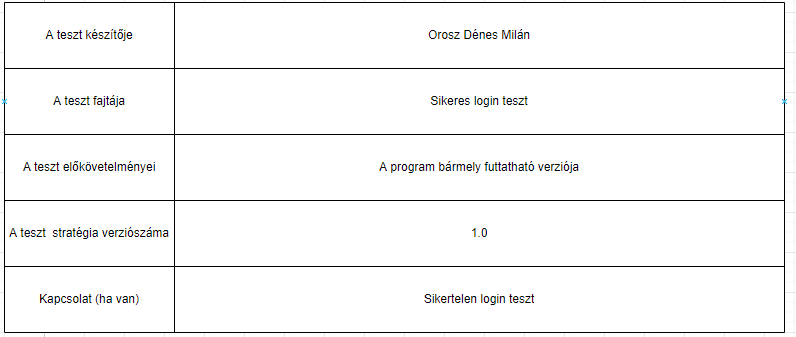
\includegraphics[scale=0.86]{images/test_case_template.png}
	\caption{A teszt esethez tartozó információk.}
	\label{fig:template}
\end{figure}
Minden teszt eset 3 vagy 4 oszlopból áll. Az első oszlopban a lépés sorszáma, a másodikban  maga a lépés van megfogalmazva, a harmadik és negyedik oszlop pedig az elvárt eredményt, illetve a lépéshez tartozó bemenetet tartalmazzák, viszont előfordulhat, hogy a bemeneteket egy másik táblázatban tárolják. Példát erre a \aref{fig:testcase} mutatja be.\\

\begin{figure}[h]
	\centering
	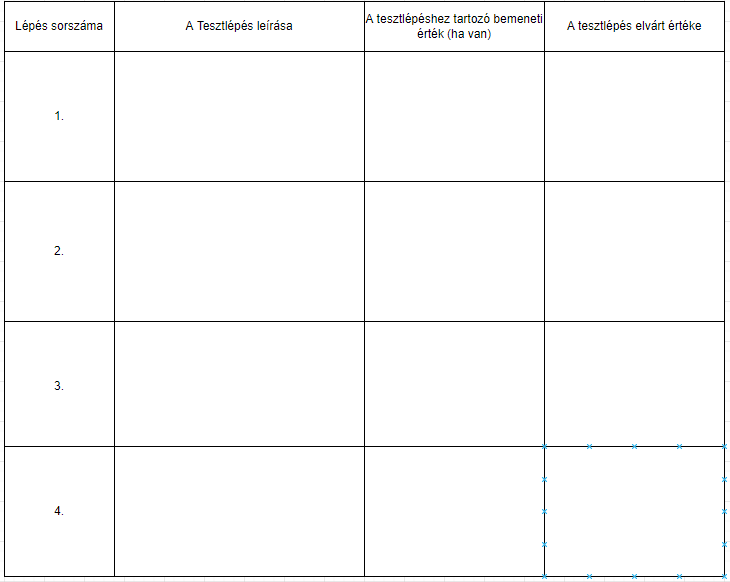
\includegraphics[scale=0.86]{images/test_case.png}
	\caption{Egy teszt eset teszt lépések nélkül}
	\label{fig:testcase}
\end{figure}



\begin{figure}
	\centering
	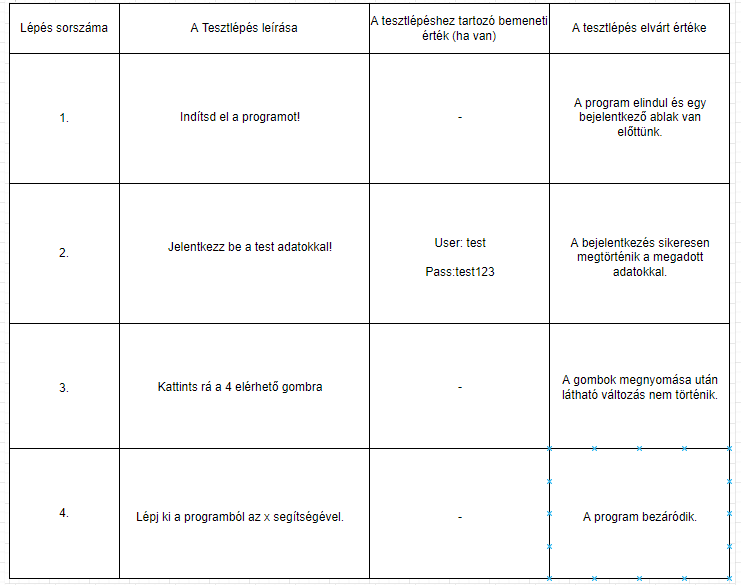
\includegraphics[scale=0.86]{images/success_login_test_case.png}
	\caption{A programhoz tartozó sikeres bejelentkezés teszt esete}
	\label{fig:successcase}
\end{figure}

A \aref{fig:successcase} képen látható, az én programomhoz tartozó bejelentkezést tesztelő teszt esetnek a lépéssorozata és a hozzá tartozó bemenetek és az elvárt eredmények.

\Chapter{Megvalósítás}

Ez a fejezet mutatja be a megvalósítás lépéseit.
Itt lehet az esetlegesen előforduló technikai nehézségeket említeni.
Be lehet már mutatni a program elkészült részeit.

Meg lehet mutatni az elkészített programkód érdekesebb részeit.
(Az érdekesebb részek bemutatására kellene szorítkozni.
Többségében a szöveges leírásnak kellene benne lennie.
Abból lehet kiindulni, hogy a forráskód a dolgozathoz elérhető, azt nem kell magába a dolgozatba bemásolni, elegendő csak behivatkozni.)

A dolgozatban szereplő forráskódrészletekhez külön vannak programnyelvenként stílusok.
Python esetében például így néz ki egy formázott kódrészlet.
\begin{python}
import sys

if __name__ == '__main__':
    pass
\end{python}

A stílusfájlok a \texttt{styles} jegyzékben találhatók.
A stílusok között szerepel még C++, Java és Rust stílusfájl.
Ezek használatához a \texttt{dolgozat.tex} fájl elején \texttt{usepackage} paranccsal hozzá kell adni a stílust, majd a stílusfájl nevével megegyező környezetet lehet használni.
További példaként C++ forráskód esetében ez így szerepel.
\begin{cpp}
#include <iostream>

class Sample : public Object
{
    // An empty class definition
}
\end{cpp}
Stílusfájlokból elegendő csak annyit meghagyni, amennyire a dolgozatban szükség van.
Más, C szintaktikájú nyelvekhez (mint például a JavaScript és C\#) a Java vagy C++ stílusfájlok átszerkesztésére van szükség.
(Elegendő lehet csak a fájlnevet átírni, és a fájlban a környezet nevét.)

Nyers adatok, parancssori kimenetek megjelenítéséhez a \texttt{verbatim} környezetet lehet használni.
\begin{verbatim}
$ some commands with arguments
1 2 3 4 5
$ _
\end{verbatim}

A kutatás jellegű témáknál ez a fejezet gyakorlatilag kimaradhat.
Helyette inkább a fő vizsgálati módszerek, kutatási irányok kaphatnak külön-külön fejezeteket.

\Chapter{Tesztelés}

A fejezetben be kell mutatni, hogy az elkészült alkalmazás hogyan használható.
(Az, hogy hogyan kell, hogy működjön, és hogy hogy lett elkészítve, az előző fejezetekben már megtörtént.)

Jellemzően az alábbi dolgok kerülhetnek ide.
\begin{itemize}
\item Tesztfuttatások. Le lehet írni a futási időket, memória és tárigényt.
\item Felhasználói kézikönyv jellegű leírás. Kifejezetten a végfelhasználó szempontjából lehet azt bemutatni, hogy mit hogy lehet majd használni.
\item Kutatás kapcsán ide főként táblázatok, görbék és egyéb részletes összesítések kerülhetnek.
\end{itemize}

\Chapter{Összefoglalás}


\section{Értékelés} A dolgozat célja a szoftver tesztelés bemutatása volt. Ez alatt értendő, hogy milyen tesztelési módszereket mikor érdemes használni és, hogy mik ezek a módszerek.\\

A szakdolgozatban számos módszerrel találkozhattunk, amiket szöveges leírás után gyakorlati példával is bemutattam, így egy átfogóbb képet kaptunk a módszerekről.
Készült egy adatbázist kezelő program a szakdolgozat mellé, aminek a célja a módszerek alkalmazása a gyakorlatban volt, így számos funkció ennek megfelelően készült el, ami lehetséges, hogy egy cégnek készült szoftverben teljesen máshogy lenne implementálva.\\

A tervezettnél a programban az adatbázissal összeköttetéssel foglalkozó funkciók jobban készültek el. Sikerült egy funkciót megírni, ami le tudja kezelni önmagában a különböző parancsokat, ahelyett, hogy parancsonként külön-külön funkcióra legyen szükség.\\

A tervezettnél rosszabbul a fa struktúra elkészítése sikerült. Szerettem volna, hogy adatbázis független legyen a program és bármilyen hozzácsatolt adatbázissal működjön, viszont végül a tesztelés szempontjából, jobbnak láttam, hogyha egy hozzá elkészített adatbázissal foglalkozik csak a program.

\section{További tervek} Mindenképpen szeretném tovább fejleszteni a programot. A tervek közé tartozna, hogy lehessen vele adatbázist kreálni és törölni, így teljesen adatbázis függetlenné tenni a programot, illetve több adatbázissal is szeretném, ha tudna egyszerre foglalkozni.\\

Ezen felül szeretnék a grafikus felületen szépíteni, illetve még plusz elemeket hozzáadni, így a jelenlegi 4 gombos rész helyett, egy teljes panelt hozzáadni a jobb széléhez, ahol ezek a gombok elérhetőek lennének és a felszabadult helyen, pedig az éppen megnyitott adatbázis elemeit lehetne látni.



\clearpage

\addcontentsline{toc}{chapter}{Irodalomjegyzék}
\bibliographystyle{unsrt}
\bibliography{dolgozat.bib}

\newpage

\pagestyle{empty}

\noindent \textbf{\Large CD Használati útmutató}

\vskip 1cm

Ennek a címe lehet például \textit{A mellékelt CD tartalma} vagy \textit{Adathordozó használati útmutató} is.

Ez jellemzően csak egy fél-egy oldalas leírás.
Arra szolgál, hogy ha valaki kézhez kapja a szakdolgozathoz tartozó CD-t, akkor tudja, hogy mi hol van rajta.
Jellemzően elég csak felsorolni, hogy milyen jegyzékek vannak, és azokban mi található.
Az elkészített programok telepítéséhez, futtatásához tartozó instrukciók kerülhetnek ide.

A CD lemezre mindenképpen rá kell tenni
\begin{itemize}
\item a dolgozatot egy \texttt{dolgozat.pdf} fájl formájában,
\item a LaTeX forráskódját a dolgozatnak,
\item az elkészített programot, fontosabb futási eredményeket (például ha kép a kimenet),
\item egy útmutatót a CD használatához (ami lehet ez a fejezet külön PDF-be vagy MarkDown fájlként kimentve).
\end{itemize}


\end{document}
